\documentclass[aspectratio=43]{beamer}
\usepackage[english]{babel}
\definecolor{beamer@blendedblue}{rgb}{0.9, 0.8,0.3}
\setbeamertemplate{footline}{\insertframenumber/\inserttotalframenumber}
\usepackage{graphicx}
\usepackage{subcaption}
\captionsetup{compatibility=false}
\usetheme{Hannover}
\usepackage{amssymb}
\usepackage{amsmath}
\usepackage{enumerate}
\usepackage{stmaryrd}
\usepackage[ruled,linesnumbered]{algorithm2e}

\begin{document}
\title{Consistency Metric for Distributed Datastores}
\author{Kyrylo Rukkas, Galyna Zholtkevych}
\institute{V.N. Karazin Kharkiv National University, Ukraine}
\date{{\bfseries International Conference Taapsd -- 2017}\\
	Kyiv, 4 -- 8 Dec 2017} 
% 
\frame{\titlepage} 
\begin{frame}{Agenda}
\begin{itemize}
\item Motivation:

\begin{itemize}
\item need to make consistent datastores
\item consistency problem of a distributed datastorage
\item need to present consistency state as stochastic value.
\end{itemize}

\item Background:

\begin{itemize}
\item eventual consistency definition;
\item consistency model expanded with new definitions;
\end{itemize}

\item Formula to define inconsistency state. Example
\item Graphics for inconsistency stochastic value
\item Consistency convergence proposition. Proof
\item Graphics for consistency convergence value
\item Conclusions and future work

\end{itemize}
\end{frame}


\begin{frame}{Motivation}
\begin{itemize}
\item Consistency is not a new problem in datastores, especially if they are huge
\item At this point in large DS it become more usable to present consistency state as stoschastic value.

\end{itemize}
\end{frame}

\begin{frame}{Background}
\begin{block}{ACID vs BASE strategy}
\begin{itemize}
\item ACID (Atomic, Consistent, Isolated, Durable) mean that once a transaction is complete, its data is consistent and stable on disk
\item BASE (Basic Availability, Soft-State, Eventual Consistency) values availability, but 
does not offer guaranteed consistency of replicated data at write time
\end{itemize}

\end{block}

\begin{block}{Eventual consistency definition}
Consistency is called eventual if no updates
take place for a long time and all replicas will gradually become consistent
\end{block}

\end{frame}

\begin{frame}{Evolved model for consistency}
Our model is a tuple $(N, L, \partial,D, r)$, where \\

$N$ -- a finite set of nodes; \\
$L$ -- a finite set of links; \\
$\partial:L\rightarrow 2^N$ -- a mapping that associates each link with two nodes;\\
$D$ -- a finite set of stored data units;\\
$r:D\rightarrow 2^N$ -- a mapping that associates each data unit $d$ with a subset of nodes 
that store its replica.
$N_d$ -- a finite set of nodes that are having given dataunit $d$; \\
$l(N_d)$ -- a number of nodes in datastore that are having given dataunit; \\
$n_c$ -- a number of nodes in a subset of $N_d$ where all nodes have the same replica.

\end{frame}

\begin{frame}{Formula and example}
\begin{block}{Consistency formula derivation}
\begin{equation}
	p_c = \frac{n_c}{l(N_d)} \cdot \frac{n_c - 1}{l(N_d) - 1}
\end{equation}
\begin{equation}\label{eq:metric}
	I(d)=1-\sum_{k=1}^K\dfrac{N_k(N_k-1)}{N(N-1)}.
\end{equation}

\end{block}
\begin{block}{Example}

\begin{tabular}{lclcl}
	$I(5)=0$ \\ $I(4+1)=\frac{2}{5}$ & & $I(3+2)=\frac{3}{5}$\\
	$I(3+1+1)=\frac{7}{10}$ && $I(2+2+1)=\frac{4}{5}$ \\
    $I(2+1+1+1)=\frac{9}{10}$\\
	$I(1+1+1+1+1)=1$
\end{tabular}

\end{block}
\end{frame}

\begin{frame}{Demonstration of experiments}
\begin{figure}
\begin{subfigure}{0.3\linewidth}
\centering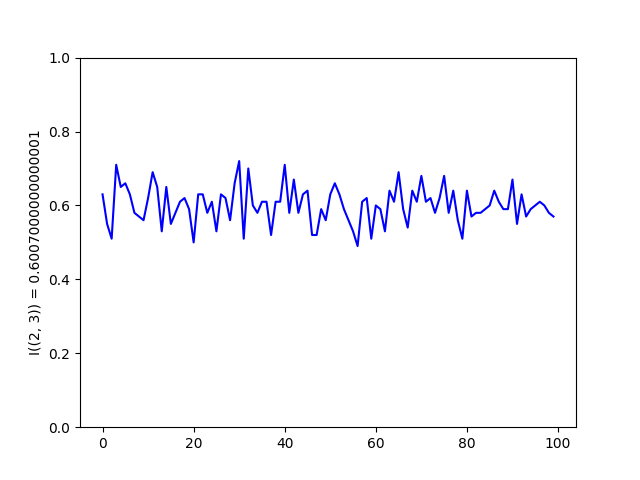
\includegraphics[width=\linewidth]{images/2-3-consistent-partitions-probability.png}\hfill
\end{subfigure}
\begin{subfigure}{0.3\linewidth}
\centering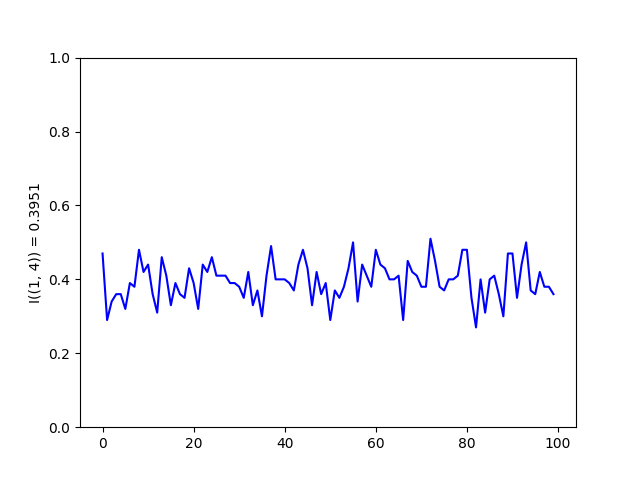
\includegraphics[width=\linewidth]{images/1-4-consistent-partitions-probability.png}
\end{subfigure}
\caption{The datastore has two consistent partitions}
\end{figure}

\begin{figure}[p]
\begin{subfigure}{0.3\linewidth}
\centering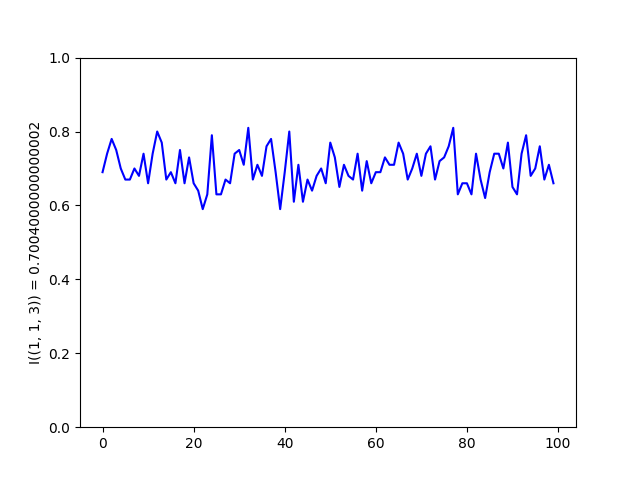
\includegraphics[width=\linewidth]{images/1-1-3-consistent-partitions-probability.png}
\end{subfigure}
\begin{subfigure}{0.3\linewidth}
\centering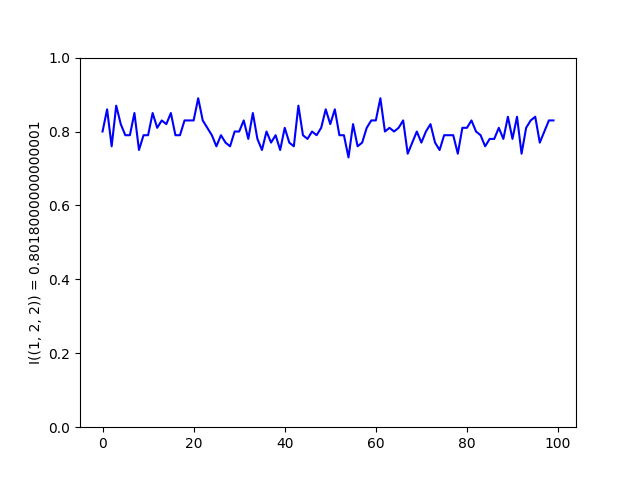
\includegraphics[width=\linewidth]{images/1-2-2-consistent-partitions-probability.png}
\end{subfigure}
\caption{The datastore has three consistent partitions}
\end{figure}

\end{frame}


\begin{frame}{Proposition about consistency convergence}
Let we have a distributed datastore where all links are available and reliable (network partitions do not happen in a datastore and nodes are stable and respond in approximately equal time); the interval between writing operations is $t_w$.
Then $t_w$ is less than the diameter of network graph ensures eventual consistency of the datastore.
\begin{block}{Brief proof}
\begin{enumerate}
\item $n_1$, $n_2$ are outermost each from other
\item Time slots $t$ taken from $n_1$ to $n_2$ is the shortest path from $n_1$ to $n_2$
\item From definition of the diameter $T_c = diameter(G)$
\end{enumerate}
\end{block}
\end{frame}

\begin{frame}{Demonstration of experiments}
\begin{figure}[p]
\begin{subfigure}{0.4\linewidth}
\centering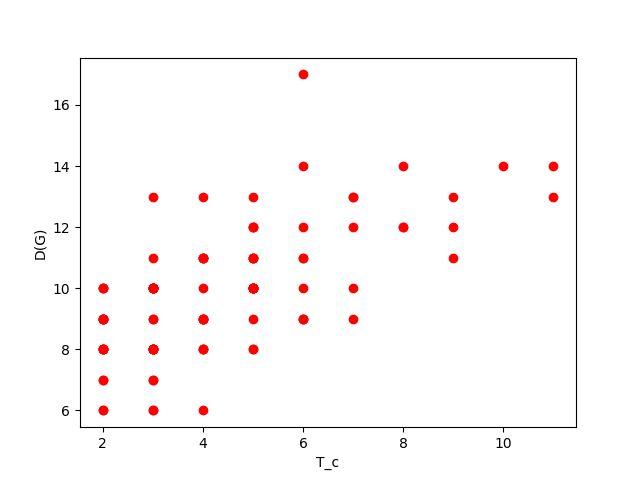
\includegraphics[width=\linewidth]{images/100-consistency-convergence-weighted.png}
\end{subfigure}
\begin{subfigure}{0.4\linewidth}
\centering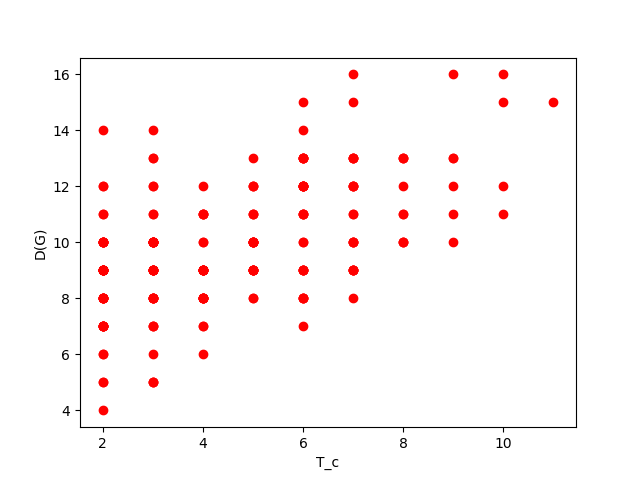
\includegraphics[width=\linewidth]{images/200-consistency-convergence-weighted.png}
\end{subfigure}
\begin{subfigure}{0.4\linewidth}
\centering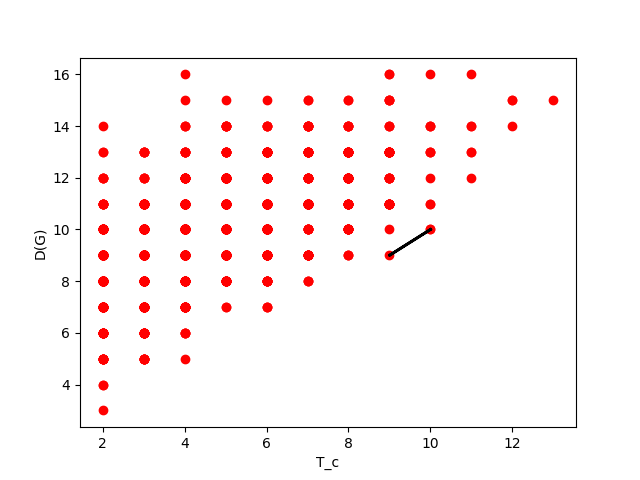
\includegraphics[width=\linewidth]{images/1000-consistency-convergence-weighted.png}
\end{subfigure}
\caption{Graphics for consistency convergence time on weighted graph}
\end{figure}

\end{frame}

\begin{frame}{Activity diagram of simulation process}

\begin{figure}
\centering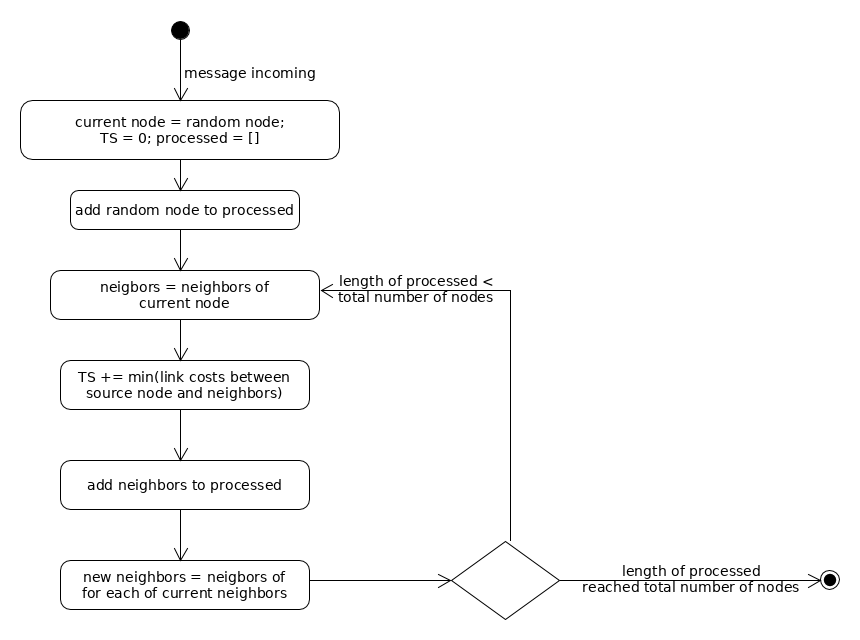
\includegraphics[width=\linewidth]{images/message-broadcasting-state-machine.png}
\end{figure}

\end{frame}

\begin{frame}{Conclusions}

\begin{itemize}
\item the sufficient condition for distributed datastore can be choosing network topology where frequency of write operations will be no greater than diameter of the graph;
\item if frequency of write operations is grater than diameter of the graph, it may be useful to evaluate current inconsistency state of the graph;
\item if inconsistency state is close to 0 enough for current requirements, it means that there are inconsistent nodes that are far enough to not conflict with new replicas. The next source can be chosen from consistent list and far enough for inconsistent ones;
\item if still more strict consistency needs to be satisfied and inconsitency state is close enough to 0, the node closest to the source node where previous write operation occurred can be chosen for writing;
\item if replica's history is not important for requirements, it may be possible to solve the problem fixing conflicts.
\end{itemize}

\end{frame}

\begin{frame}{Future work}
\begin{itemize}
\item complicate a datastore introducing different availability for each node;
\item complicate a datastore introducing various network partitions for a datastore;
\item provide an algorithm that will allow to make a decision what is the best approach for a given datastore such that the eventually consistency is satisfied or an approach when inconsistency will not impact on datastore requirements;
\item theory for finding the most actual replica and time complexity for this algorithm
\item consider all the proposed above metrics in various kinds of real topologies.
\end{itemize}

\end{frame}


\end{document}